\section{Overview}

Chapter~\ref{chap:integration} briefly summarizes the system developed
and documented in the previous chapters. Various measurements are
reproduced and interpreted in system context.

\begin{figure}[htbp]
\begin{center}
	\includegraphics*{whole-system2.ps}
	\caption{Active electrode EEG acquisition system.}
\label{fig:eeg-fin}
\end{center}
\end{figure}

Figure~\ref{fig:eeg-fin} is a photograph of the final EEG data
acquisition system prototype. Figure~\ref{fig:eeg-fin} shows the
active electrode container mounted on the SME physical model. The AE
container is wore in the same manner as depicted in the photograph
while measuring EEG signals from a human subject.

The blue metal box houses the LLSPM electronics as well as the power
pack for the whole system. The connecting power and signal cables are
fastened unto the foam-rubber strip of the SAM container with short
Velcro strips. 


\section{System Integration}

\begin{figure}[htbp]
\begin{center}
	\psfrag{ae1}[][]{$ae_1$}
	\psfrag{ae2}[][]{$ae_2$}
	\psfrag{rld}[][]{RLD}
	\psfrag{e}[][]{$e$}
	\psfrag{dc}[][]{DC}
	\psfrag{dif}[][]{IA}
	\psfrag{hp}[][]{HP}
	\psfrag{lp}[][]{LP}
	\psfrag{dis}[][]{HLSP}
	\psfrag{sc}[][]{SC}
	\psfrag{a}[][]{$a$}
	\psfrag{b}[][]{$b$}
	\psfrag{c}[][]{$c$}
	\psfrag{d}[][]{$d$}
	\psfrag{e}[][]{$e$}
	\psfrag{f}[][]{$f$}
	\psfrag{g}[][]{$g$}
	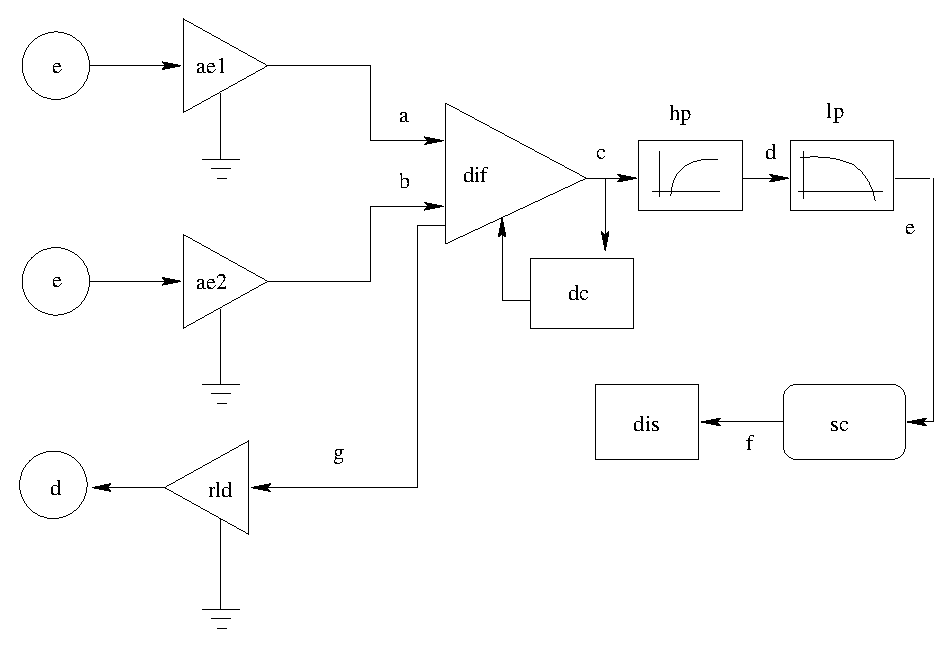
\includegraphics[width=\textwidth]{integration.eps}
	\caption{System integration block diagram.}
\label{fig:integration}
\end{center}
\end{figure}

Figure~\vref{fig:integration} describes the system data flow in block
diagram format. The EEG - common mode signal combination is extracted
from the physical electrodes ($e$). The signal is buffered by the
active electrodes ($ae_1$ and $ae_2$) and the common mode signal
subtracted from the EEG signal with the instrumentation amplifier
IA. The resulting signal is filtered through the high-pass (HP) and
low-pass (LP) filters before being digitized in the SC module
(SC). For clarity the amplifiers described in
Section~\ref{secion:llspm-amp} has been lumped with their associated
filters.

The mean of the difference signal between $a$ and $b$ is fed back to
the skin surface via the right leg drive circuit (RLD). The AD620
output signal at $c$ is sampled and the DC value fed back to the AD620
reference pin to reduce the DC component of the signal at $c$. The
HLSPM is implemented by the PicoScope visualization software used
throughout this report.

The design and implementation of each module and submodule is
documented in the preceding chapters.

\section{Measurements}

\begin{figure}[htbp]
\begin{center}
	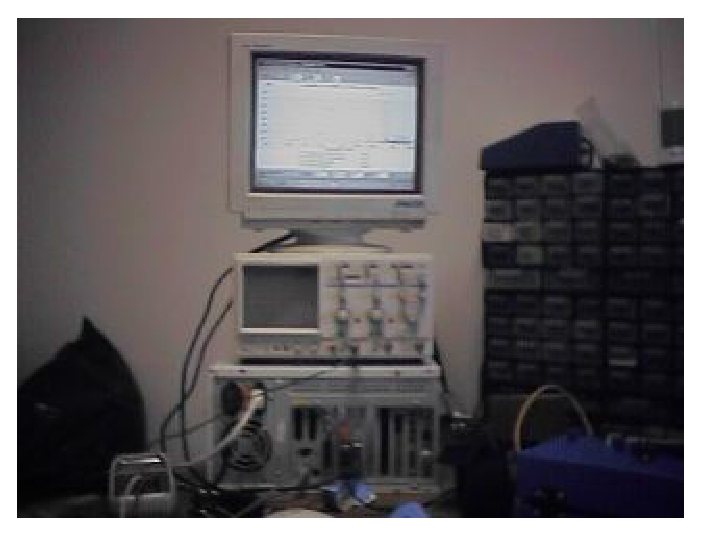
\includegraphics{test-setup.ps}
	\caption{Test and measurement environment.}
\label{fig:test+measure}
\end{center}
\end{figure}
 
Figure~\ref{fig:test+measure} is photograph of the test environment
used during the development and evaluation of the system. The bottom
component is a 133~MHz Pentium PC running Windows~98 and the PicoScope
visualization tools. The ADC-42 is plugged into a open parallel port
in front and easily accessible. The middle component is 20~MHz dual
channel oscilloscope. 

All graphical records of time and frequency plots documented in this
report were generated with a ADC-42 ADC system. The PicoScope
visualization software were used to generate the graphics in WMF
format (Windows Meta Format). WMF files were converted to encapsulated
postscript files (eps) using the Gimp\footnote{http://www.gimp.org}
for inclusion into the \LaTeX~source document.


\subsection{Noise and interference}
\begin{figure}[htbp]
\begin{center}
	\psfrag{r1}[][]{$R_1$}
	\psfrag{r2}[][]{$R_2$}
	\psfrag{r3}[][]{$R_3$}
	\psfrag{a}[][]{a}
	\psfrag{b}[][]{b}
	\psfrag{c}[][]{c}
	\psfrag{d}[][]{d}
	\psfrag{ae1}[][]{$ae_1$}
	\psfrag{ae2}[][]{$ae_2$}
	\psfrag{drv}[][]{drive}
	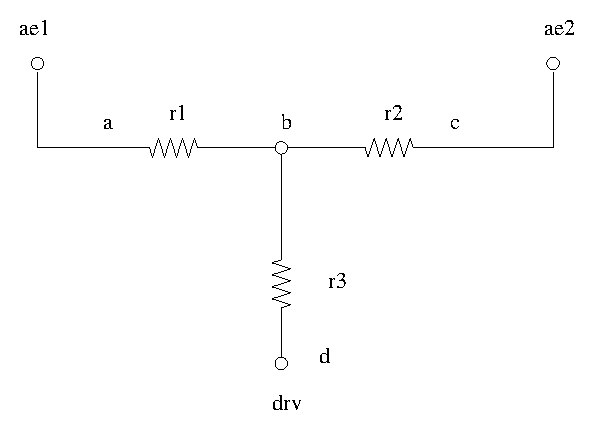
\includegraphics{noise-m.eps}
	\caption{System noise measurement configuration.}
\label{fig:noise-m}
\end{center}
\end{figure}

For system noise measurements the system input were configured as
depicted in Figure~\vref{fig:noise-m}. The resistances $R_1$, $R_2$,
and $R_3$ are used to simulate electrode resistance for worst--case
conditions ($R_1 = R_2 = R_3 = 100~k\Omega$) as well as optimal
conditions ($R_1 = R_2 = R_3 = 0~\Omega$).

\subsubsection{Passive System noise level measurement}

In order to determine the amount of noise generated internally by a
active system a passive system interference measurement is first
required. A comparison between active and passive system noise may
give additional insight into the sources of noise and interference. 

The goal of a passive noise investigation is to take cognizance of
present levels of noise or interference and employ active or passive
techniques to reduce the measured noise levels. Preventing signal
noise contamination before it occurs is far easier than removing noise
from a contaminated signal.

The system is connected in the manner described by the test
configuration of Figure~\ref{fig:noise-m}. The inputs of $ae_1$ and
$ae_2$ is shorted together and directly connected to the output of the
RLD ($d$), that is $R_1 = R_2 = R_3 = 0~\Omega$. The EEG system is left
in a powered--down state and the measurement taken at the low--pass
output ($e$).

\begin{figure}[htbp]
\begin{center}
	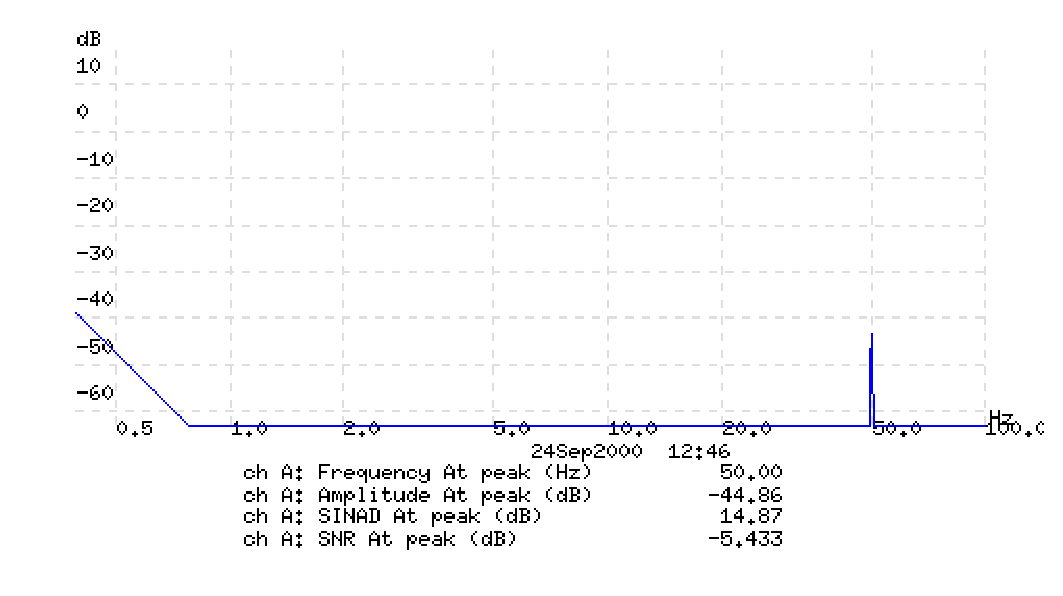
\includegraphics[width=\textwidth]{SEEGNS1.ps}
    \caption{EEG System passive noise}
    \label{fig:eegnoise-passive}
\end{center}
\end{figure}


Figure~\ref{fig:eegnoise-passive} describes the output as seen at node
$f$ in Figure~\ref{fig:integration} for the powered--down system with
all passive noise shielding deployed. That is, the system is housed in
its metal container and the electrode cables are shielded as
previously described.

A 256 sample Hanning window was used to create the spectrum of
Figure~\ref{fig:eegnoise-passive}. The only visible component is a
-44.86~dB 50~Hz interference signal. This measurement indicates that
the EEG system passive EMI shielding is effective.


\subsubsection{Active system noise level measurements}

Subsequent noise measurements involves the system in a powered--up
state. The goal of an active noise investigation is to determine the
level of internal or active component noise the system contributes to
the detected EEG signal. Once this level of noise is known a measure
of the integrity of the signal can be made. 

\subsubsection{Worse case active noise levels ($100~k\Omega$ electrode resistance)}
For worst--case noise levels it is assumed that the skin resistance
between the active electrode surface and the tissue below the stratum
granulossum is 100~k$\Omega$. The effect of the RLD circuit is also
investigated.


\begin{figure}[htbp]
\begin{center}
	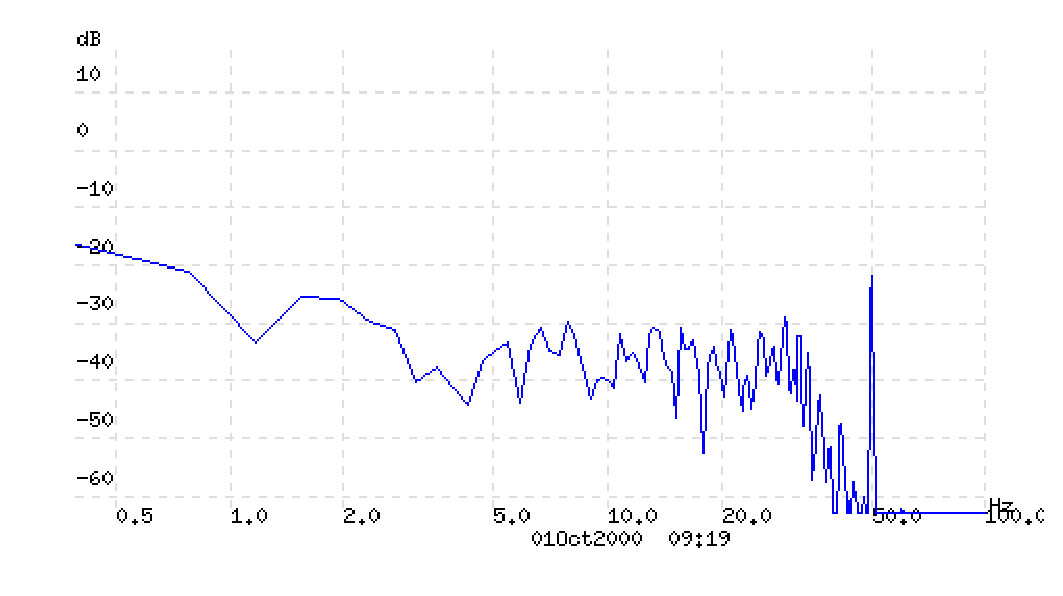
\includegraphics[width=\textwidth]{N2ON100K.ps}
    \caption{$R_1$ = $R_2$ = 100~k$\Omega$ electrode resistance}
    \label{fig:N2ON100K}
\end{center}
\end{figure}

Figure~\ref{fig:N2ON100K} is a trace of the system output signal at
$f$ in Figure~\ref{fig:integration}. The electrodes are connected in
the configuration specified in Figure~\ref{fig:noise-m} with $R_1$ =
$R_2$ = $R_3$ = 100~k$\Omega$. The RLD is connected to d. From
Figure~\ref{fig:N2ON100K} can be seen that the mean noise floor lies
at approximately -30~dB, a -23~dB 50~Hz interference signal is also
present. 


\begin{figure}[htbp]
\begin{center}
	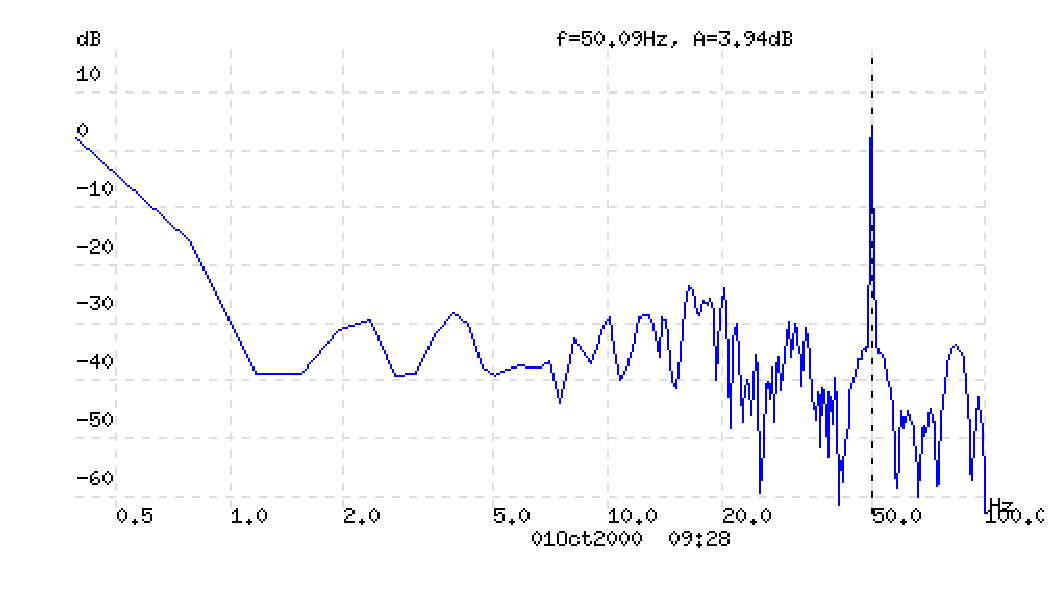
\includegraphics[width=\textwidth]{N3NRLD1.ps}
    \caption{$R_1$ = $R_2$ = 100~k$\Omega$, RLD deactivated}
    \label{fig:N3NRLD1}
\end{center}
\end{figure}

Figure~\ref{fig:N3NRLD1} is a trace of the system output signal at $f$
in Figure~\ref{fig:integration}. The electrodes are connected in the
configuration specified in Figure~\ref{fig:noise-m} with $R_1$ = $R_2$
= 100~k$\Omega$. The RLD is disconnected from d. From
Figure~\ref{fig:N3NRLD1} can be seen that the mean noise floor is not
affected significantly if compared with that of
Figure~\ref{fig:N2ON100K}, that is level at approximately -30~dB. It
is however clear that the 50~Hz spike is significantly larger
($\pm$20~dB). There is also a extra high frequency noise component to
the right of the 50~Hz spike.


\begin{figure}[htbp]
\begin{center}
	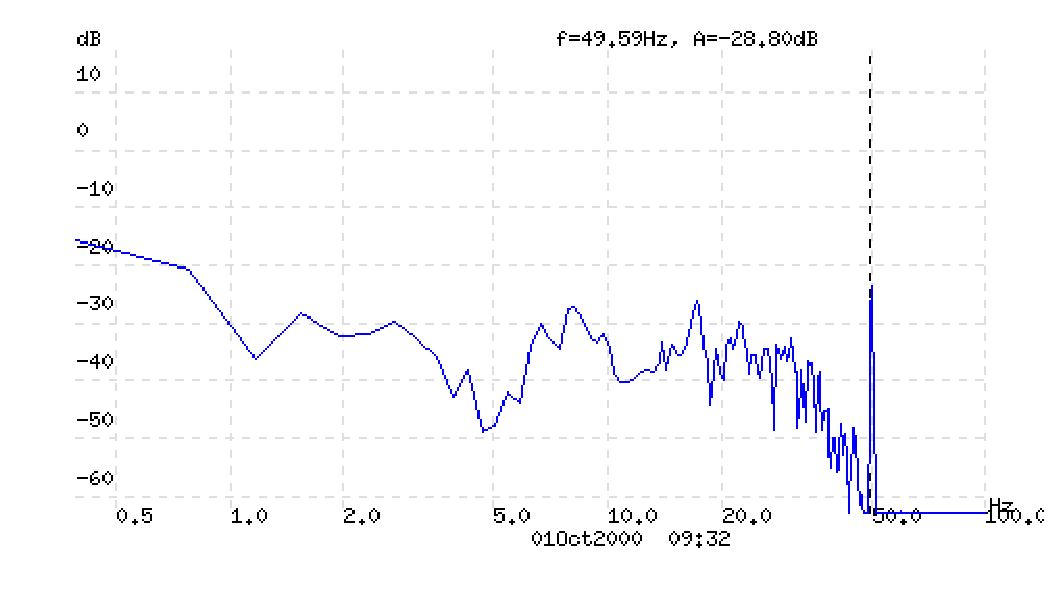
\includegraphics[width=\textwidth]{N4RLD1.ps}
    \caption{$R_1$ = $R_2$ = 100~k$\Omega$, $R_3$ = 0~$\Omega$, RLD activated}
    \label{fig:N4RLD1}
\end{center}
\end{figure}

Figure~\ref{fig:N4RLD1} is a trace of the system output signal at $f$
in Figure~\ref{fig:integration}. The electrodes are connected in the
configuration specified in Figure~\ref{fig:noise-m} with $R_1$ = $R_2$
= 100~k$\Omega$ and $R_3$ = 0~$\Omega$. The RLD is connected to
d. Figure~\ref{fig:N4RLD1} is resembles Figure~\ref{fig:N2ON100K} both
in terms of the mean noise floor as well as the amplitude of the 50~Hz
spike. As expected the electrode resistance of the RLD does not
influence the effectiveness of the RLD. 


\begin{figure}[htbp]
\begin{center}
	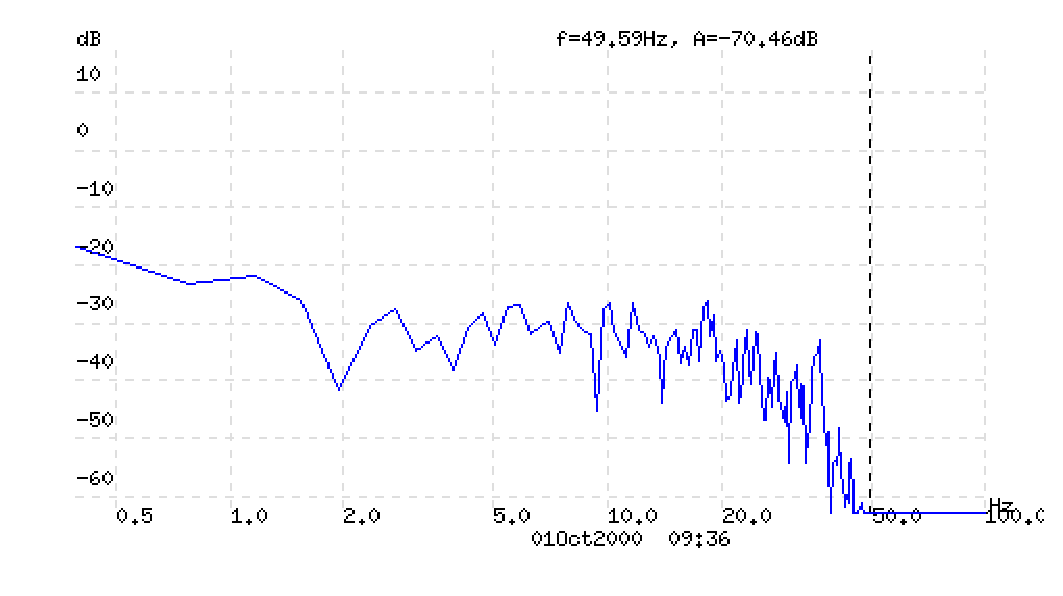
\includegraphics[width=\textwidth]{N5RLD.ps}
    \caption{$R_1$ = $R_2$ = 0~k$\Omega$, $R_3$ = 0~$\Omega$, RLD activated}
    \label{fig:N5RLD1}
\end{center}
\end{figure}

Figure~\ref{fig:N5RLD1} is a trace of the system output signal at $f$
in Figure~\ref{fig:integration}. The electrodes are connected in the
configuration specified in Figure~\ref{fig:noise-m} with $R_1$ = $R_2$
= 0~k$\Omega$ and $R_3$ = 0~$\Omega$. The RLD is connected to d. This
configuration represents ideal noise conditions and is unlikely to be
encountered during normal system operation. From
Figure~\ref{fig:N5RLD1} can be seen that the 50~Hz signal is heavily
attenuated (-70.46~dB). This result is expected as the effectiveness
of the RLD circuit is dependent on the electrode source resistances.


\begin{figure}[htbp]
\begin{center}
	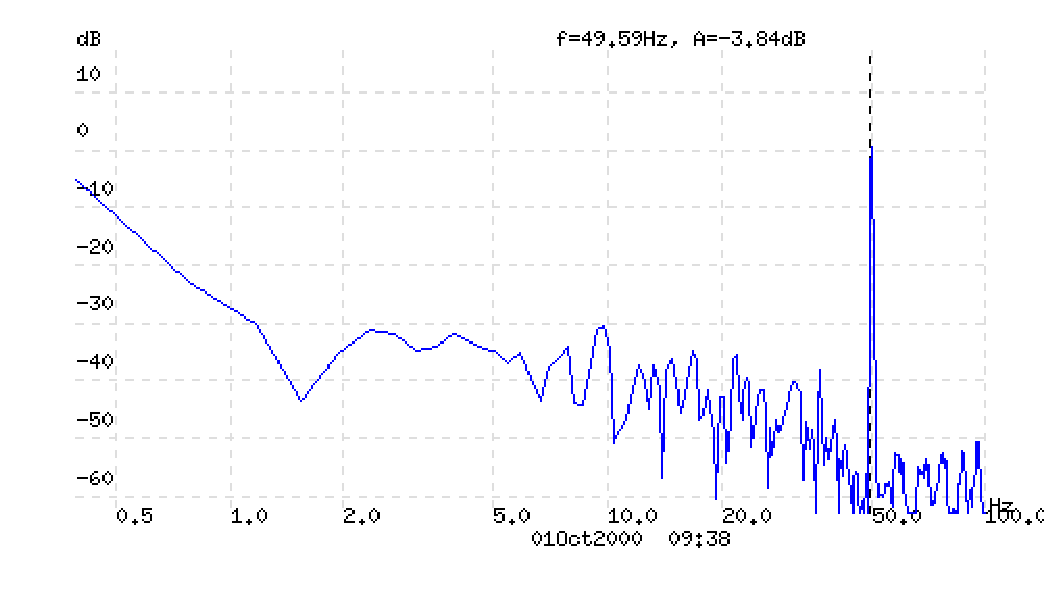
\includegraphics[width=\textwidth]{N6NRLD.ps} \caption{$R_1$ =
    $R_2$ = 0~k$\Omega$, $R_3$ = 0~$\Omega$, RLD deactivated}
    \label{fig:N6RLD1}
\end{center}
\end{figure}

Figure~\ref{fig:N6RLD1} is a trace of the system output signal at $f$
in Figure~\ref{fig:integration}. The electrodes are connected in the
configuration specified in Figure~\ref{fig:noise-m} with $R_1$ = $R_2$
= 0~k$\Omega$ and $R_3$ = 0~$\Omega$. The RLD is disconnected. As is
expected the 50~Hz interference signal is severe, even for 0~$\Omega$
source resistances. Once again higher frequency noise is visible to
the left of the 50~Hz spike.

\subsection{SME measurements}
All SME test signals were used during the final evaluation of the EEG
system. The $\alpha$ SME test signal evaluation is documented below.

\begin{figure}[htbp]
\begin{center}
	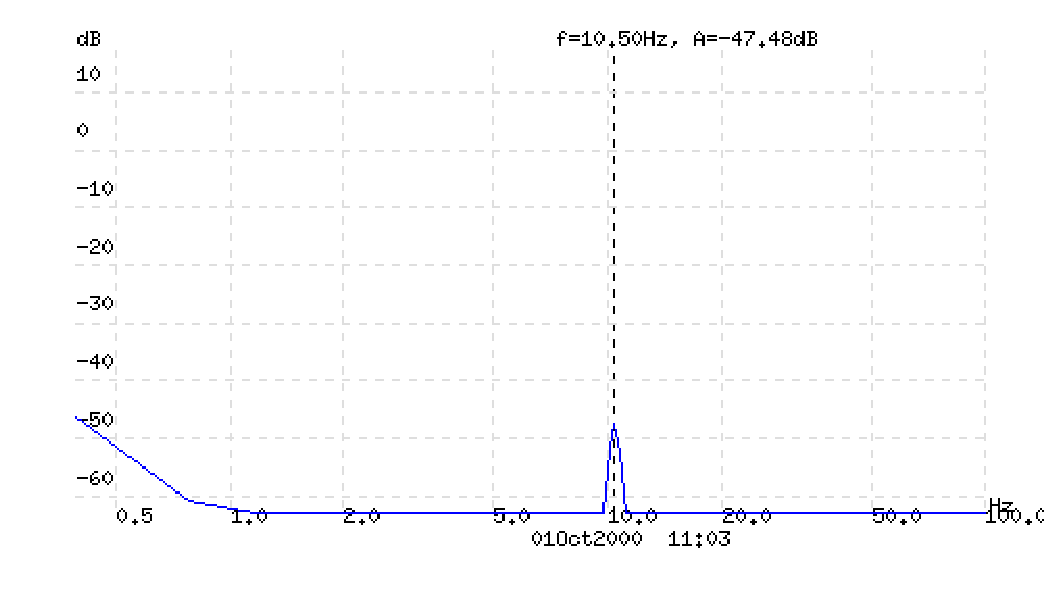
\includegraphics[width=\textwidth]{LOW10.ps} 
	\caption{SME $\alpha$ (10~Hz) test signal}
    \label{fig:LOW10}
\end{center}
\end{figure}

Figure~\ref{fig:LOW10} is the output of the $\alpha$ SME signal
generator. The signal was further reduced in amplitude by a voltage
divider before injected into the EEG system. The output of the AD620
was monitored and the signal amplitude reduced until it was no longer
discernible on the oscilloscope.


\begin{figure}[htbp]
\begin{center}
	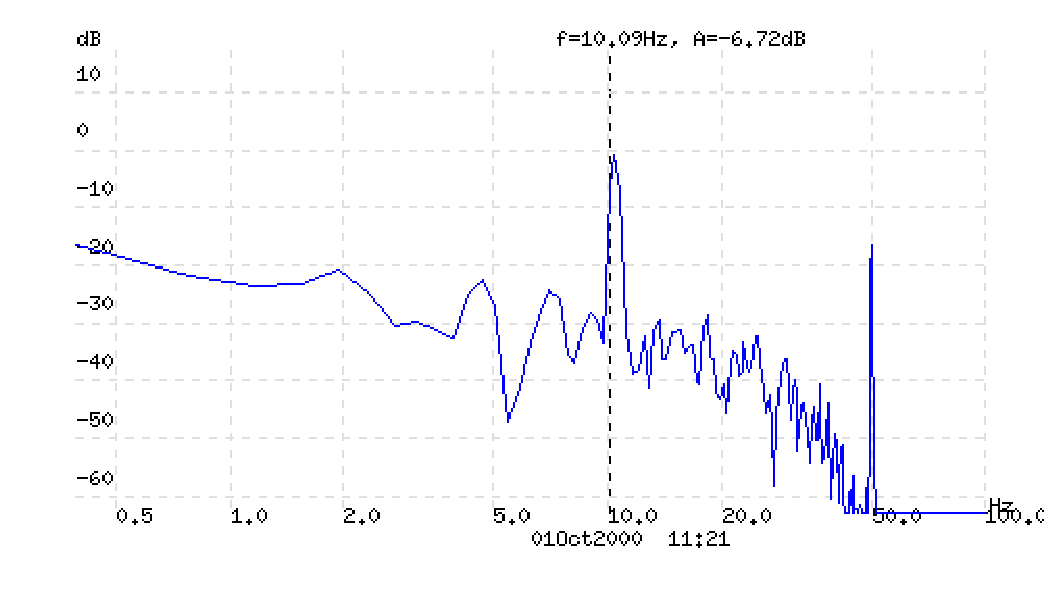
\includegraphics[width=\textwidth]{SME10LOW.ps} 
	\caption{$R_1$ = $R_2$ = $R_3$ = 10~k$\Omega$, SME $\alpha$ (10~Hz) test signal}
    \label{fig:SME10LOW}
\end{center}
\end{figure}

Figure~\ref{fig:SME10LOW} is a trace of the system output signal at
$f$ in Figure~\ref{fig:integration} with a injected SME $\alpha$ test
signal. The electrodes are connected in the configuration specified in
Figure~\ref{fig:noise-m} with $R_1$ = $R_2$ = $R_3$ =
10~k$\Omega$. The RLD is connected to d. The injected $\alpha$ signal
is clearly discernible in Figure~\ref{fig:SME10LOW}. 


\begin{figure}[htbp]
\begin{center}
	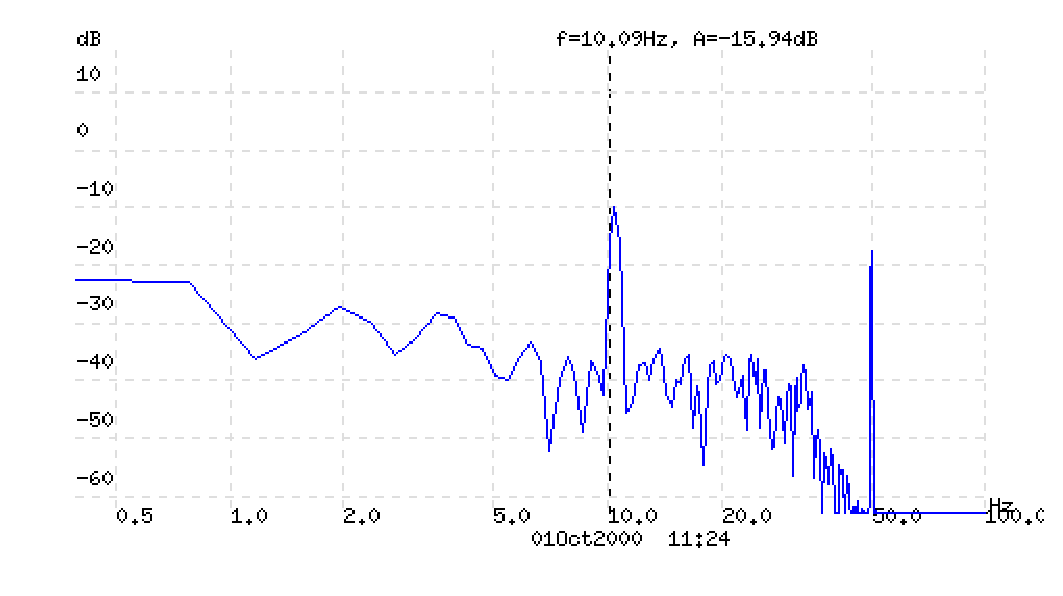
\includegraphics[width=\textwidth]{SME10LOW2.ps} 
	\caption{$R_1$ = $R_2$ = 10~k$\Omega$, $R_3$ = 0~$\Omega$, 
	SME $\alpha$ (10~Hz) test signal}
    \label{fig:SME10LOW2}
\end{center}
\end{figure}

Figure~\ref{fig:SME10LOW2} is a trace of the system output signal at
$f$ in Figure~\ref{fig:integration} with a injected SME $\alpha$ test
signal. The electrodes are connected in the configuration specified in
Figure~\ref{fig:noise-m} with $R_1$ = $R_2$ = 10~k$\Omega$ and $R_3$ =
0~$\Omega$. The RLD is connected to d. The RLD experiment is repeated
with the same result as previously except for the drop in $\alpha$
amplitude (-6.72~dB to -15.94~dB). This can be explained by the
reduction in input resistance of the voltage divider used to inject
the test signal. This explanation is however not completely
satisfactorily.

\subsection{$F_{p1}$, $F_{p2}$ measurements}
The goal of the $F_{p1}$, $F_{p2}$ measurements is to verify that the
system is indeed measuring EEG signals and not noise. The two graphs
of $F_{p1}$, $F_{p2}$ measurements given below were measured over a
ten minute period and represent typical values from the system.

\begin{figure}[htbp]
\begin{center}
	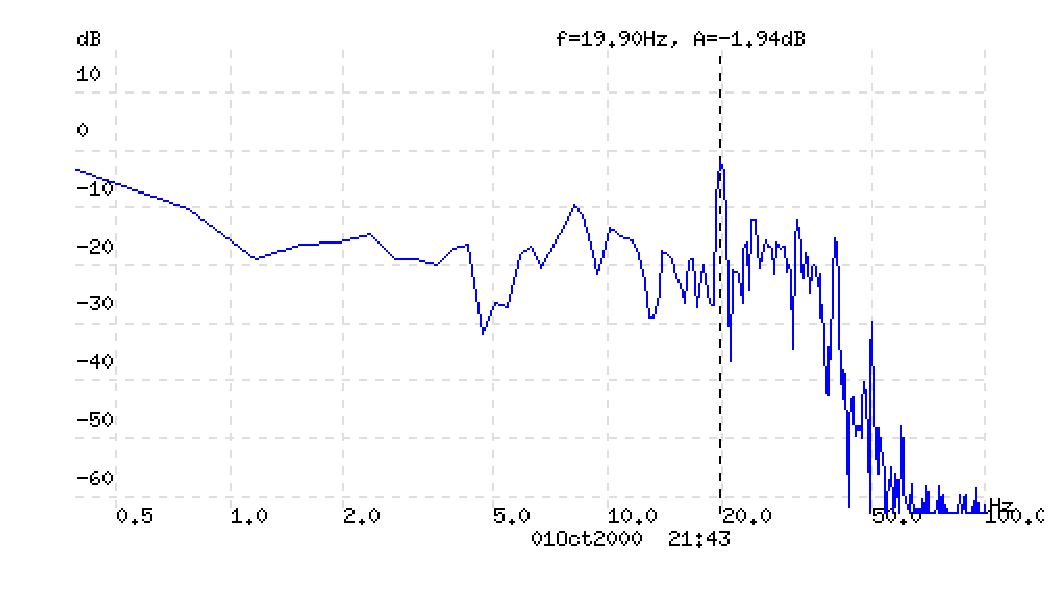
\includegraphics[width=\textwidth]{EEG1.ps} 
	\caption{$F_{p1}$, $F_{p2}$, RLD right ear}
    \label{fig:EEG1}
\end{center}
\end{figure}

Figure~\ref{fig:EEG1} is a trace of the system output signal at $f$ in
Figure~\ref{fig:integration} with the active electrodes connected to
the $F_{p1}$ and $F_{p2}$ international montage positions. The RLD
earth electrode was clipped to the subject's right ear. A small
(-48~dB) 50~Hz interference signal is present. A sharp peak (-1.94~dB)
at 20~Hz is present.

\begin{figure}[htbp]
\begin{center}
	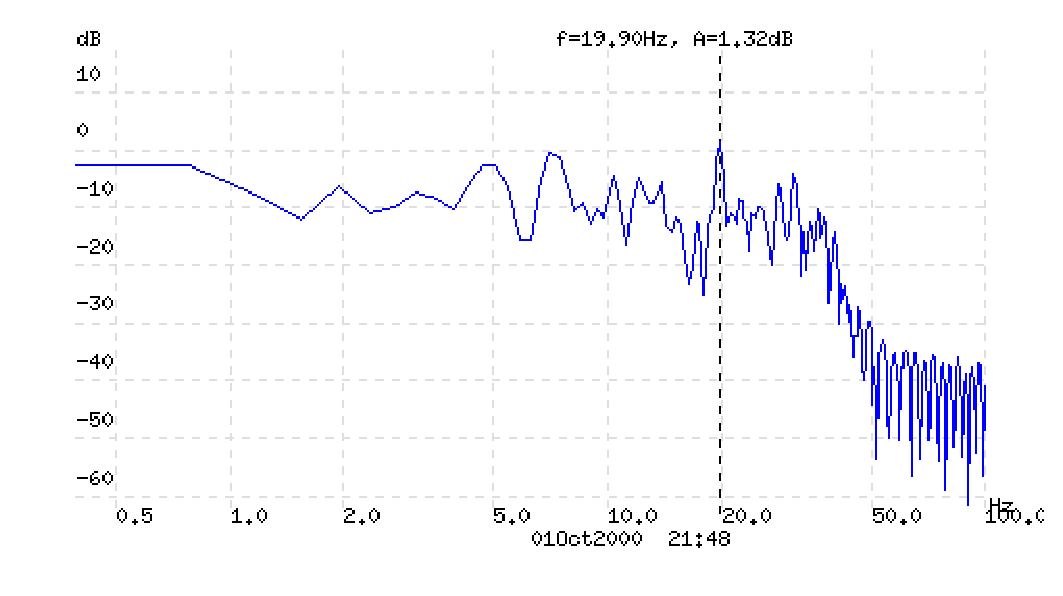
\includegraphics[width=\textwidth]{EEG2.ps} 
	\caption{$F_{p1}$, $F_{p2}$, RLD left ear}
    \label{fig:EEG4}
\end{center}
\end{figure}

Figure~\ref{fig:EEG2} is a trace of the system output signal at $f$ in
Figure~\ref{fig:integration} with the active electrodes connected to
the $F_{p1}$ and $F_{p2}$ international montage positions. The RLD
earth electrode was clipped to the subject's left ear. 

Various positions for the RLD electrode was used, although some
differences in the scalp signal were noticed depending on the position
of the RLD electrode it did not seem to be significant. In this
measurement the noise floor is significantly higher (30~dB) than the
right ear RLD measurement.

\subsubsection{Visual processing test}
In order to test whether the system is capable of detecting the
difference between open--eye and closed--eye readings an average scalp
signal measurement over two 60~s periods were made.


\begin{figure}[htbp]
\begin{center}
	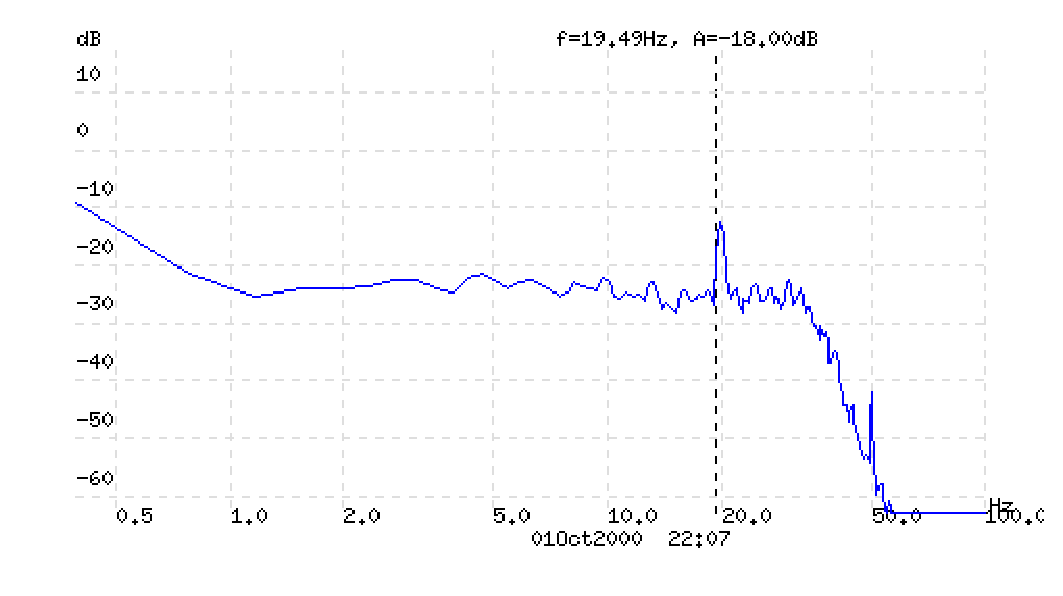
\includegraphics[width=\textwidth]{EEGAV3TOE.ps} 
	\caption{Eyes closed 60~s averaging period}
    \label{fig:EEGAV3TOE}
\end{center}
\end{figure}

Figure~\ref{fig:EEGAV3TOE} is a trace of the system output signal at
$f$ in Figure~\ref{fig:integration} with the active electrodes
connected to the $F_{p1}$ and $F_{p2}$ international montage
positions. The RLD earth electrode was clipped to the subject's right
ear. The scalp signal were averaged for a period of 60~s while the
subject kept his eyes closed.


\begin{figure}[htbp]
\begin{center}
	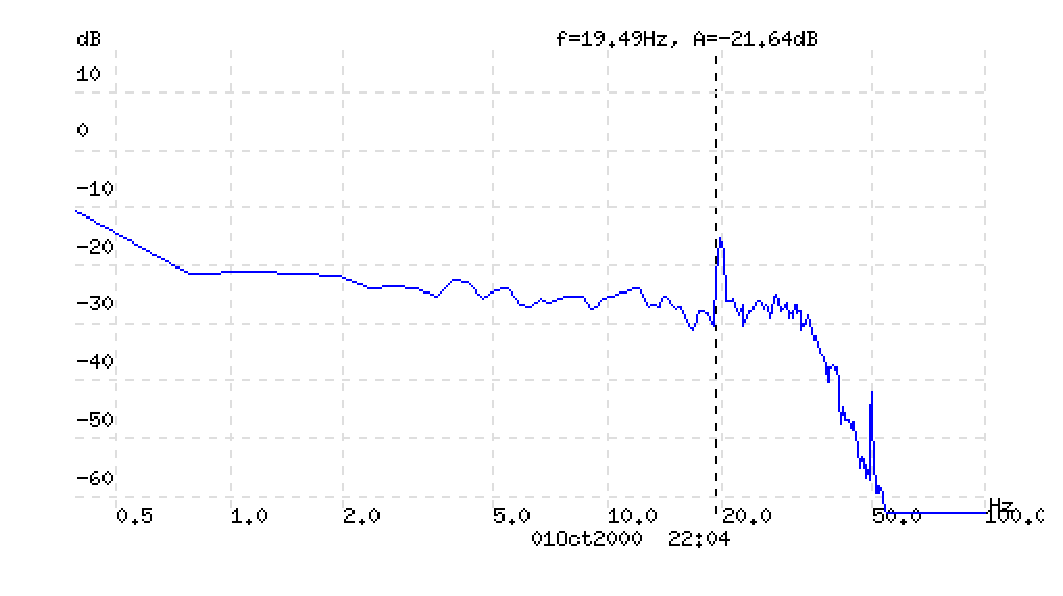
\includegraphics[width=\textwidth]{EEGAV3OOP.ps} 
	\caption{Eyes open 60~s averaging period}
    \label{fig:EEGAVOOP}
\end{center}
\end{figure}

Figure~\ref{fig:EEGAVOOP} is a trace of the system output signal at
$f$ in Figure~\ref{fig:integration} with the active electrodes
connected to the $F_{p1}$ and $F_{p2}$ international montage
positions. The RLD earth electrode was clipped to the subject's right
ear. The scalp signal were averaged for a period of 60~s while the
subject kept his eyes open.

It was expected that the average amplitude of the open--eyes graph be
higher than that of the closed--eye test. The opposite is the case,
the close--eye graph has a slightly higher signal average. 

It was noticed that the average signal trace does drop or climb
momentarily when the subject closes his eyes or opens them. It is
suspected that this is due to ocular artifacts and not EEG signal
amplitude.

\subsubsection{Binaural Beats test}

A binaural audio test was attempted to test whether the system can
detect the so--called 'brain
entrainment'\footnote{http://www.psid.com/radiosonic.net/eeg\_article.htm}
phenomenon in which a specific frequency in the EEG range can be
stimulated by using binaural beats.

For the binaural beat test 10~Hz were chosen as the beat frequency and
300~Hz as the carrier frequency. The
Sbagen\footnote{http://www.aguazul.demon.co.uk/bagen/} tool was used
to produce the beat.


\begin{figure}[htbp]
\begin{center}
	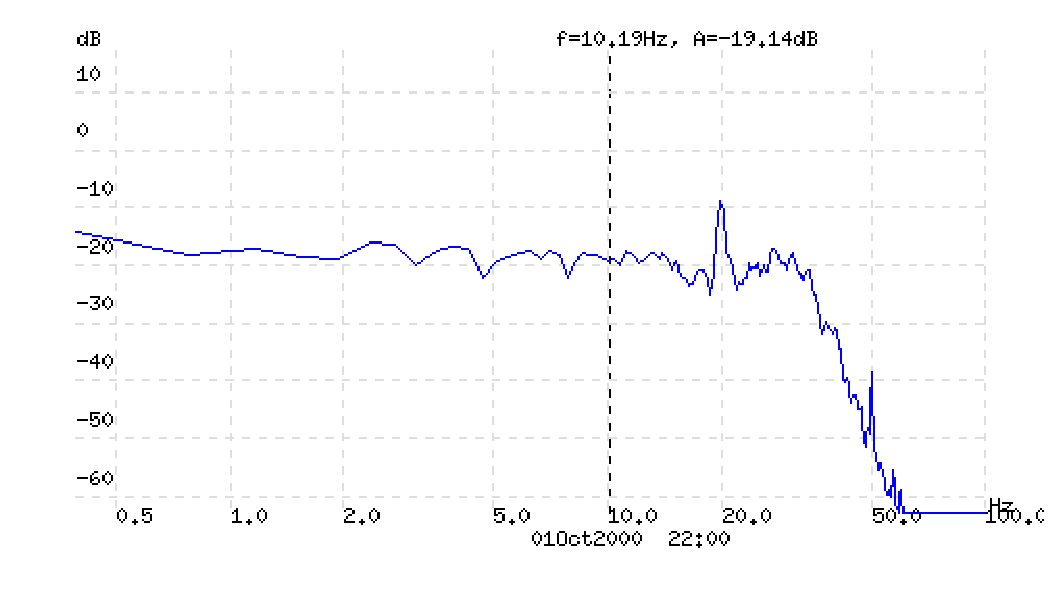
\includegraphics[width=\textwidth]{EEGAV2.ps} 
	\caption{Binaural beat on}
    \label{fig:EEGAV1}
\end{center}
\end{figure}

Figure~\ref{fig:EEGAV1} is a trace of the system output signal at $f$
in Figure~\ref{fig:integration} with the active electrodes connected
to the $F_{p1}$ and $F_{p2}$ international montage positions. The RLD
earth electrode was clipped to the subject's right ear. The scalp
signal were averaged for a period of 60~s while the subject listened
to a 10~Hz binaural beat.

\begin{figure}[htbp]
\begin{center}
	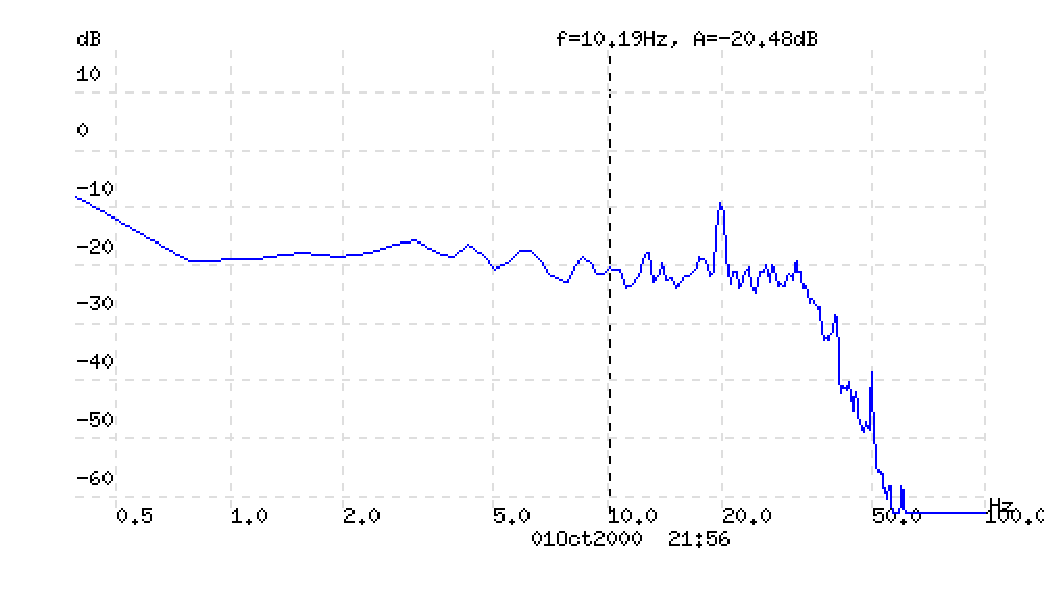
\includegraphics[width=\textwidth]{EEGAV1.ps} 
	\caption{Binaural beat off}
    \label{fig:EEGAV2}
\end{center}
\end{figure}

Figure~\ref{fig:EEGAV2} is a trace of the system output signal at $f$
in Figure~\ref{fig:integration} with the active electrodes connected
to the $F_{p1}$ and $F_{p2}$ international montage positions. The RLD
earth electrode was clipped to the subject's right ear. The scalp
signal were averaged for a period of 60~s while the subject listened
to pink noise.

A small (2~dB) difference between the two measurements were detected
over the measurement period. This difference is well within the normal
variance (3~dB) of the rest of the signal. A similar test over a
longer averaging period (10~minutes) had a slightly larger difference
but still inconclusive.

\section{Conclusion}

While most of the quantitative tests that the system and the system's
modules were subjected to suggests that an active electrodes system can
be a feasible alternative to a traditional passive electrode based
system, the qualitative tests were inconclusive.

It will be necessary to compare a the system with another proven
system having a identical LLSPM subsystem in order to make a
comparative analysis. Alternatively the LLSPM, which was the bulk of
the project, must be abandoned and a commercial system adapted to make
use of active electrodes.




